\documentclass[a4paper, margin=1in]{article}
%\usepackage{CJK}
\usepackage{latexsym}
\usepackage{color}
\usepackage[x11names]{xcolor} % for a set of predefined color names, like LemonChiffon1
\usepackage{graphicx, float}\usepackage{graphicx}
\usepackage{algorithm}
\usepackage{algpseudocode}
\usepackage{mathtools}
\usepackage{hyperref}
\usepackage[toc,page]{appendix}
\usepackage{bm}
\usepackage{pdfpages}
\setlength{\oddsidemargin}{-0.0in}
\setlength{\evensidemargin}{-0.0in} \setlength{\textwidth}{6.0in}
\setlength{\textheight}{9.0in} \setlength{\topmargin}{-0.2in}
%\usepackage[boxruled]{algorithm2e}

%\setlength{\leftmargin}{0.7in}
\usepackage{amssymb, graphicx, amsmath}  %  fancyheadings,
\usepackage{setspace}
\newcommand\qed{\qquad $\square$}
\newcommand{\nn}{\nonumber}

\usepackage{lipsum}

\usepackage{listings}
\lstset{
  basicstyle=\ttfamily,
  columns=fullflexible,
  frameround=fttt,
  breaklines=true,
  %postbreak=\mbox{\textcolor{red}{$\hookrightarrow$}\space},
}

\definecolor{mGreen}{rgb}{0,0.6,0}
\definecolor{mGray}{rgb}{0.5,0.5,0.5}
\definecolor{mPurple}{rgb}{0.58,0,0.82}
\definecolor{backgroundColour}{rgb}{0.95,0.95,0.92}

\lstdefinestyle{CStyle}{
basicstyle=\ttfamily,
language=C,
numberstyle=\tiny\color{mGray},
numbers=left,
frame=lines,
framexleftmargin=0.5em,
framexrightmargin=0.5em,
backgroundcolor=\color{LemonChiffon1},
showstringspaces=false,
escapeinside={(*@}{@*)},
}

\def \[{\begin{equation}}
\def \]{\end{equation}}
\def\proof{{\bf Proof:\quad}}
\def \endzm {\quad $\Box$}
\def\dist{\hbox{dist}}

\usepackage{tabularx,booktabs}
\newcolumntype{C}{>{\centering\arraybackslash\hsize=.5\hsize}X} % centered version of "X" type
\setlength{\extrarowheight}{1pt}
\usepackage{caption}% <-- added


\newcommand{\R}{\mathbb{R}}
%\newtheorem{yinli}{����}[section]
\newcommand{\D}{\displaystyle}
\newcommand{\T}{\textstyle}
\newcommand{\SC}{\scriptstyle}
\newcommand{\FT}{\footnotesize}

\usepackage{hyperref}
\newcommand\fnurl[2]{%
  \href{#2}{#1}\footnote{\url{#2}}%
}


%\newtheorem{theorem}{Theorem}[section]
%\renewcommand{\thetheorem}{\arabic{section}.\arabic{theorem}}
\newtheorem{definition}{Definition}
\renewcommand{\thedefinition}{\arabic{section}.\arabic{definition}}
\newtheorem{lemma}{Lemma}[section]
\renewcommand{\thelemma}{\arabic{section}.\arabic{lemma}}
\newtheorem{remark}{Remark}
\renewcommand{\theremark}{\arabic{section}.\arabic{remark}}
\newtheorem{proposition}{Proposition}[section]
\renewcommand{\theproposition}{\arabic{section}.\arabic{proposition}}
\newtheorem{corollary}{Corollary }[section]
\renewcommand{\thecorollary}{\arabic{section}.\arabic{corollary}}
\renewcommand{\theequation}{\arabic{section}.\arabic{equation}}
\renewcommand{\baselinestretch}{1.35}
\newtheorem{exam}{Example}[section]
\renewcommand{\theexam}{\arabic{section}.\arabic{exam}}
\newtheorem{theo}{Theorem}[section]
\renewcommand{\thetheo}{\arabic{section}.\arabic{theo}}

\usepackage{enumitem}
\newenvironment{QandA}{\begin{enumerate}[label=\bfseries\alph*.]\bfseries}
	{\end{enumerate}}
\newenvironment{answered}{\par\normalfont}{}

% Define a \HEADER{Title} ... \ENDHEADER block
\makeatletter
\newcommand{\HEADER}[1]{\ALC@it\underline{\textsc{#1}}\begin{ALC@g}}
\newcommand{\ENDHEADER}{\end{ALC@g}}
\makeatother

\newcommand{\argmin}{\operatornamewithlimits{argmin}}
\newcommand{\argmax}{\operatornamewithlimits{argmax}}

\usepackage{url} % to make url in bibtex shows up

% Create a command to cleanly insert a snippet with the style above anywhere in the document
\newcommand{\insertcode}[2]{\begin{itemize}\item[]\lstinputlisting[caption=#2,label=#1,style=CStyle]{#1}\end{itemize}} % The first argument is the script location/filename and the second is a caption for the listing

\DeclarePairedDelimiter\abs{\lvert}{\rvert}
\DeclarePairedDelimiter\floor{\lfloor}{\rfloor}
\DeclarePairedDelimiter\ceiling{\lceil}{\rceil}

\begin{document}
%\begin{CJK*}{GBK}{song}

\begin{center}

{\LARGE \bf CS380L: Advanced Operating Systems Lab \#3}\\

\vskip 25pt
 {Zeyuan Hu \footnote{30 hours spent on this lab.}, iamzeyuanhu@utexas.edu }\\
\vskip 5pt
{\small EID:zh4378 Spring 2019 }

\end{center}

\begin{spacing}{1.5}
\section{Environment} \label{environment}

Unless otherwise noted, we use a Linux server for all the experiments. The server has 4 Intel(R) Xeon(R) CPU E3-1220 v5 @ 3.00GHz processors and 16GB of memory, and runs Ubuntu 16.04.2 LTS (kernel version 4.11.0).

\section{ELF}

Executable and Linkable Format (ELF) is a file format for executable, object code, shared libraries, and core dump on UNIX-like systems  \cite{elf_wiki}. ELF format is shown in Figure \ref{elf_format}, which is taken from \cite{elf_doc}. An ELF binary 
starts with a fixed-length \textit{ELF header}, which holds a ``road map" describing the file's organization (e.g., instruction set architecture, endianness, system ABI, program's entry point). A \textit{program header table}, if present, tells the system how to create a process image (i.e., execute a program). Each entry of program header table corresponds to a segment in the virtual address space. Part of the segment contents can be loaded from the executable file, which is also defined in the program header table. A \textit{section header table} contains information describing the file's sections (e.g., \texttt{.text}, \texttt{.data}, \texttt{.rodata}, \texttt{.bss}). Some of them will be loaded into virtual address space as part of segments indicated by program header table. Each entry gives information such as section name, the section size, etc. Program header table is required for to-be-run file and optional for relocatable file; section header table is required for file used during linking and optional for others.

There are some special sections we care about in ELF. \texttt{.text} section contains the program's executable instructions; \texttt{.rodata} represents read-only data, such as ASCII string constants produced by the C compiler; \texttt{.data} holds the program's initialized data, such as global variables declared with initializers like \lstinline|int x = 5;|; \texttt{.bss} section holds uninitialized data (e.g., uninitialized global variables such as \texttt{int x};) that contribute to the program?s memory image. \texttt{.bss} immediately follows \texttt{.data} in memory. C requires that ``uninitialized" global variables start with a value of zero. Thus, the system initializes the data with zeros when the program begins to run. The section occupies no file space (linker records just the address and size of the \texttt{.bss} section). The loader or the program itself must arrange to zero the \texttt{.bss} section.

\begin{figure}
	\centering
	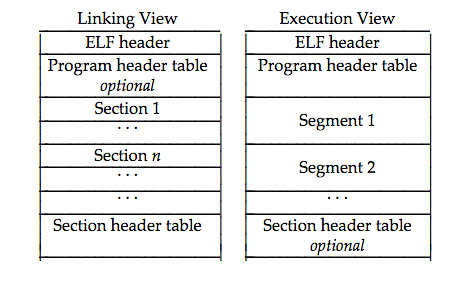
\includegraphics[scale=0.6]{elf_format.png} 
	\caption{ELF format. There are two views of ELF binary: linking view and execution view. Linking view is used during the dynamic linking, whereas execution view is needed when load the program into memory for the program to run.}
	\label{elf_format}
\end{figure}

To gather better sense of ELF, we write a simple ``Hello World" program (\lstinline|test_helloworld.c|) shown below to study its ELF content.

\begin{lstlisting}[style=CStyle]
#include <stdio.h>

int main() {
  printf("Hello world.\n");
  return 0;
}
\end{lstlisting}

We compile the program via \lstinline|gcc -static -O0 -g -std=c11 -o test_helloworld test_helloworld.c -lpthread| and then inspect its ELF content via \lstinline|readelf -l test_helloworld|. The printout of the \texttt{readelf} is shown in Figure \ref{helloworld_elf}. We see there are six segments with five kinds of \lstinline|p_type|: \lstinline|PT_LOAD|, \lstinline|PT_NOTE|, \lstinline|PT_TLS|, \lstinline|PT_GNU_STACK|, and \lstinline|PT_GNU_RELRO|. \lstinline|PT_LOAD| indicates loadable segments; \lstinline|PT_NOTE| specifies the location and size of auxiliary information; \lstinline|PT_TLS| specifies the thread-local storage template \cite{program_header}. \lstinline|PT_GNU_STACK| and \lstinline|PT_GNU_RELRO| are linux-specific \lstinline|p_type| values \cite{lsb}: \lstinline|PT_GNU_STACK| indicates whether stack is executable and \lstinline|PT_GNU_RELRO| specifies the location and size of a segment which may be made read-only after relocation shave been processed. As we will see in the following section, linux \texttt{execve} implementation mainly concerns about program header table entry with type \lstinline|PT_LOAD|.

\lstinline|readelf -l| also gives section to segment mapping. As we can see, multiple sections can be contained within the same segment. For example, the first segment contains sections like \texttt{.init} (contains the process initialization code, which is executed before calling the main program entry point), \texttt{.text}, \texttt{.rodata} and the second segment contains sections like \texttt{.data}, \texttt{.bss}. Note the second segment also contains \lstinline|.init_array| and \lstinline|.fini_array|, which are pointers to functions that will be executed when program starts and ends respectively \cite{acron}. In addition, we see the memory layout starts from address \texttt{0x400000}, which is configured by linker. We need to change this address in some way for our loader program.

\begin{figure}
	\centering
	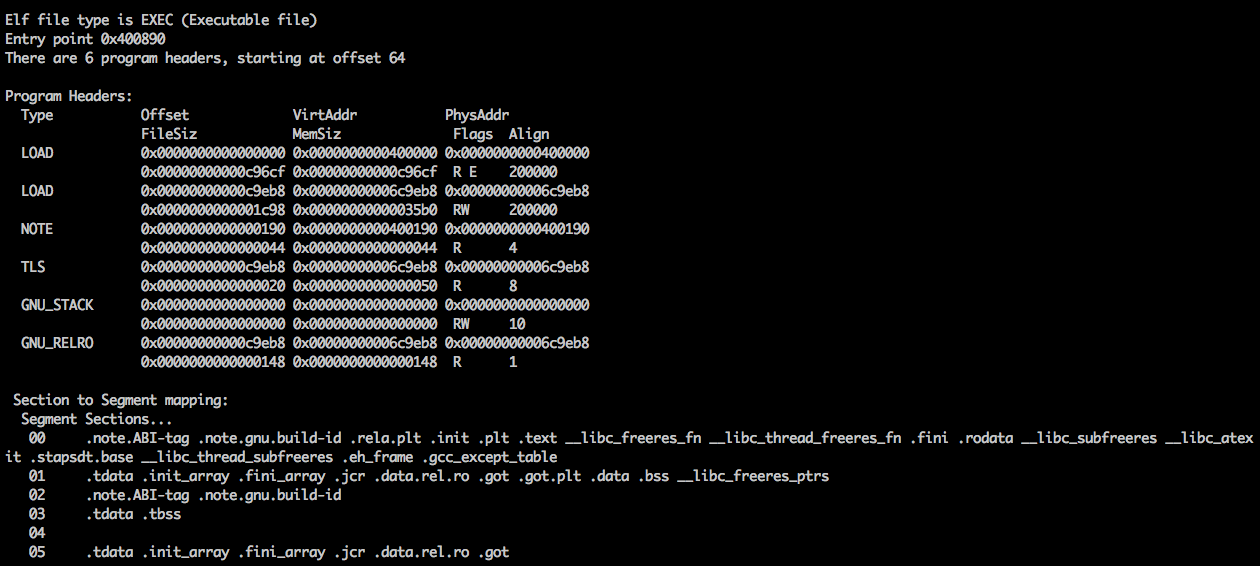
\includegraphics[scale=0.4]{helloworld_elf.png} 
	\caption{\texttt{readelf -l} printout of the \texttt{test\_helloworld} executable.}
	\label{helloworld_elf}
\end{figure}

\section{\texttt{execve} Implementation}

To write our own loader program, we first need to understand how \texttt{execve} system call is implemented in Linux kernel \footnote{we study the source code of Linux 4.8.12}. Essentially, \texttt{execve} performs the heavylifting work of loading a program into memory and start the execution of program as a process in Linux. The main logic of \texttt{execve} is implemented in \lstinline|do_execveat_common| in \texttt{fs/exec.c}. Inside \lstinline|do_execveat_common|, we see the critical function call stack looks like below:

\begin{lstlisting}[style=CStyle]
do_execveat_common
|- exec_binprm
   |- search_binary_handler
      |- load_binary
\end{lstlisting}

For binary with ELF format, \lstinline|load_elf_binary| is registered with \lstinline|load_binary| in \texttt{fs/binfmt\_elf.c}. Thus, we locate the core function \lstinline|load_elf_binary|, which is responsible to load binary with ELF format in the Linux kernel. Further study of the function reveals that the following critical steps are performed in order to load the program into memory and start execution:

\begin{itemize}
	\item Read the ELF header and perform some simple consistency checks. For example, the function checks whether the binary file is executable file (\lstinline|ET_EXEC|) or shared object file (\lstinline|ET_DYN|).
	\item Read the program header table by calling \lstinline|load_elf_phdrs|.
	\item Walk through the entries of the program header table and perform specific actions based on program header table entry type (e.g., \texttt{p\_type}). Note that \lstinline|e_phnum| holds the number of entries in the program header table. Each entry of the table corresponds to a memory segment in the binary file. Kernel is only interested in three types of program header entries during the walk through of the program header table:
	\begin{itemize}
		\item \lstinline|PT_INTERP| entry, which identifies the run-time linker needed to assemble the complete program \cite{oracle_linker}.
		\item \lstinline|PT_GNU_STACK| entry, which determines whether the program's stack should be executable \cite{lwn}.
		\item \lstinline|PT_LOPROC ... PT_HIPROC|, which are values reserved for processor-specific semantics \cite{oracle_linker}.
	\end{itemize}
	\item Once all the program header table entries have been processed, the function performs some checks based on \lstinline|p_type| value it obtained from the previous step (e.g., check for interpreter, check for specific processor architecture).
	\item The function now is ready to set up the new program. The very first step is to call \lstinline|flush_old_exec|, which clears up state in the kernel that refers to the previous program. Some minor setups (e.g., set up program's personality \cite{personality_man}) are performed immediately after. 
	\item \lstinline|setup_new_exec| is called to set up the kernel's internal state for the new program and new credentials for this executable is installed via calling \lstinline|install_exec_creds|.
	\item \lstinline|setup_arg_pages| is invoked to set up kernel's memory tracking structures (e.g., stack \lstinline|vm_area_struct|). This step is part of the goal to set up virtual memory for the new program.
	\item The function now traverse the program header table again and look for entries with type \lstinline|PT_LOAD|, which indicates loadable segments (i.e., areas of the new program's running memory). The entries contain code and data sections that come from the executable file and the size of a \texttt{BSS} section. For each \lstinline|PT_LOAD| entry, the function maps it into the process' address space via \lstinline|elf_map| call and sets up the new program's memory layout accordingly.
	\item \lstinline|set_brk| is invoked to set up zero-filled pages that correspond to the program's BSS \cite{bss} segment.
	\item \lstinline|create_elf_tables| is called to set up the rest of the new program's stack. Basically, the function puts \texttt{argc}, \texttt{argv}, \texttt{envp}, and auxiliary vectors. LWN article \cite{lwn} provides an illustration of the content of the stack set up by the kernel. In addition, Figure 3.11 of System V ABI for \lstinline|x86_64| manual \cite{abi} provides what initial process stack looks like.
	\item \lstinline|start_thread| is invoked to start the execution of the new program.
\end{itemize}
 
\section{User-space Loader}

The main goal of this lab is to construct user-space loaders. The main functionality of a loader is to copy the code and data in given executable file into memory and then run the program by jumping to its first instruction (\textit{entry point}). To organize the layout of our process memory (i.e., coexistence of memory segments for both loader program and loaded program), we check \texttt{/proc/self/maps} of the previous ``hello world" program and the output is shown below:

\begin{lstlisting}[style=CStyle]
00400000-004ca000                r-xp     00000000   fd:01    12551950   /<-snip->/test_helloworld
006c9000-006cc000                rw-p     000c9000   fd:01    12551950   /<-snip->/test_helloworld
006cc000-006ce000                rw-p     00000000   00:00    0          /<-snip->/test_helloworld
01138000-0115b000                rw-p     00000000   00:00    0          [heap]
7ffdaab86000-7ffdaaba7000        rw-p     00000000   00:00    0          [stack]
7ffdaabd6000-7ffdaabd8000        r--p     00000000   00:00    0          [vvar]
7ffdaabd8000-7ffdaabda000        r-xp     00000000   00:00    0          [vdso]
ffffffffff600000-ffffffffff601000 r-xp     00000000   00:00    0          [vsyscall]
\end{lstlisting}

There are four memory segments we need to pay attention to: the first two memory segments contain the code and data loaded from executable (e.g., \texttt{.data}, \texttt{.text}); the third segment corresponds to \texttt{.bss} section; heap follows immediately after and stack. Note, the starting address of the first memory segment is \texttt{0x400000} and stack resides in very high portion of the address space. In addition, \texttt{[vvar]}, \texttt{[vdso]}, \texttt{[vsyscall]} are not our main concern here as they are dealing with speedup of some syscall. Those observations allude our plan to organize both loader and loaded programs in a single address space as shown in Figure \ref{loader}. From the figure, one can find that we choose \texttt{0x7f400000} as the starting address of the loader program, which has an offset of \texttt{0x7f000000} from \texttt{0x400000}, which amounts to roughly 2GB  for loaded program's segment. This space is necessary as we do not support relocation (i.e., the addresses in the program headers of the loaded program are treated as fixed addresses) and we do not want two program's memory segments overlap.

To such memory organization, we need to modify the starting address of the first memory segment of our loader program, we use a linker script to tell \texttt{ld} the intended memory layout. We obtain the default linker script used by \texttt{gcc} via \texttt{ld --verbose}. We copy the default linker script to some file (e.g., \texttt{linker.lds}) and modify the following line:

\begin{lstlisting}[style=CStyle]
PROVIDE (__executable_start = SEGMENT_START("text-segment", 0x400000)); . = SEGMENT_START("text-segment", 0x400000) + SIZEOF_HEADERS;
\end{lstlisting}

by replacing \texttt{0x400000} with the desired starting address value of our loader program (e.g., \texttt{0x7f400000} in our case).

\begin{figure}[!b]
	\centering
	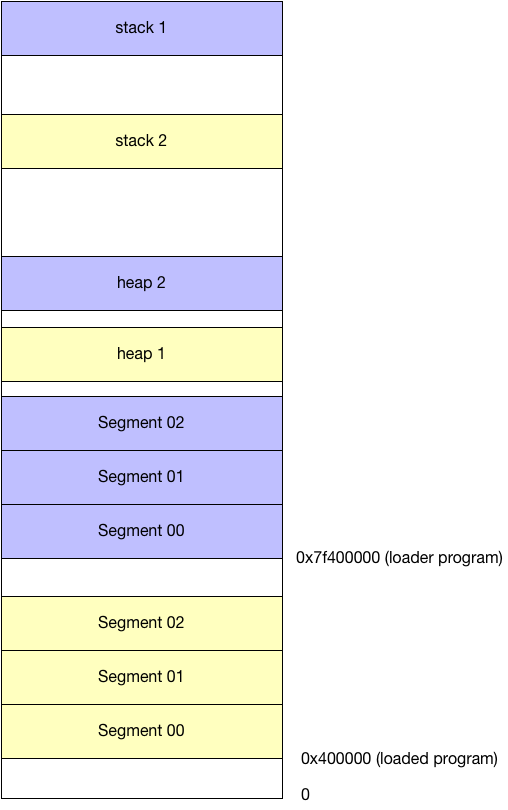
\includegraphics[scale=0.5]{loader.png} 
	\caption{Virtual address space organization of loader and loaded program}
	\label{loader}
\end{figure}

Besides process memory organization, we also need to figure out how to build loaded program's stack. Based on System V ABI for x86-64 \cite{abi}, our stack has the layout shown in Figure \ref{stack}, which is exactly same as Figure 3.11 of the manual.

\begin{figure}
	\centering
	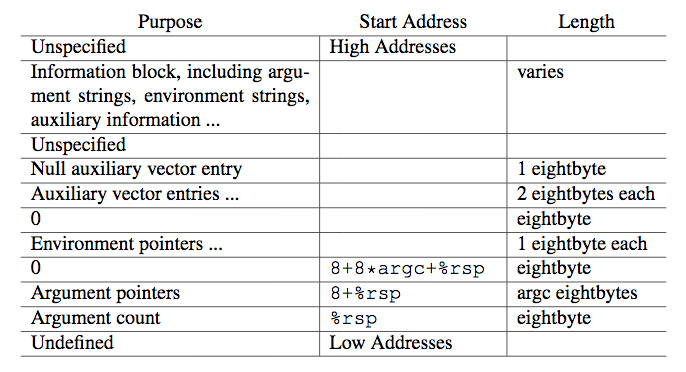
\includegraphics[scale=0.5]{stack.png} 
	\caption{Initial stack structure}
	\label{stack}
\end{figure}

Now we have all the pieces we need to build a user-space loader and the workflow looks like below:

\begin{itemize}
	\item Read and parse the ELF executable of the loaded program to extract
	necessary file header table and program header table information
	\item Load the memory segments of the loaded program into the loader's virtual address space (setup by the kernel's loader). There are three approaches: all-at-once paging, demand paging, and hybrid paging. We will discuss them in details in the following sections. For safety, we need to ensure that memory segments (except stack) of the loaded program do not go beyond \texttt{0x7f400000}.
	\item Build stack for the loaded program. Per the previous discussion, initial stack contains \texttt{argc}, \texttt{argv}, \texttt{envp}, and auxiliary vector entries. We use \texttt{mmap} to allocate space for the loaded program's stack (kernel helps to decide which to put stack in the loader's address space). Auxiliary vectors are the same ones provided by kernel to the loader. The only place we need to change is to manually setup the auxiliary vector of program headers, which should point to the loaded program's program header entries.
	\item Setup registers and jump to the entry point of the loaded program. We need to setup \texttt{\%rsp} register to point to the top of stack. In addition, we have to set \texttt{\%rdx} register to 0 as \texttt{\%rdx} is a function pointer that application should register with \texttt{atexit} \cite{abi}.
\end{itemize}

To carry out the last step, we use the following assembly embedded in C:

\begin{lstlisting}[style=CStyle]
void __attribute__((noinline)) go(void *entry, void *rsp) {
  __asm__("movq $0, %rdx;"
               "movq %rsi, %rsp;"
               "jmp *%rdi;");
}
\end{lstlisting}

Note that according to System V x86 ABI \cite{abi}, function arguments of the function is passed via registers \texttt{\%rdi} and \texttt{\%rsi} respectively.

\subsection{All-at-once loading}

In this setting, all the loaded program's memory segments are loaded into loader's address space before the execution of the loaded program.  In our implementation, memory segments are read and placed in the memory region of address space via \texttt{mmap}. The detailed description of the test programs are left to \ref{evaluation} section. We find that when \texttt{malloc}  invoked by the test program, \texttt{brk} syscall is invoked and there is no issue with test program's behavior. This is due to the fact that we setup heap segment for loaded program as well in the loader address space.

\subsection{Demand loading}

In this setting, we only map a single page of the executable under test. When segmentation fault happens, loader will first try to load the segment indicated by the faulting address. If no such segment is found, that means that a true segmentation fault happens. The loader will call \texttt{exit} to stop the execution. we use this method to preserve memory access errors. For example, for the given ``memory access errors" program in the lab description, both demand loader and the kernel loader raise the segmentation fault. If the segment indicated by the faulting address is found, loader will set up the page containing the faulting address.  Please note that in the loader, only one page will set up, not the entire segment.

Implementation-wise, we leverage \texttt{sigaction} to set up the signal handler for \texttt{SGSEGV} signal. We use a new stack for the signal handler (created using \texttt{sigaltstack}). The main reason for using another stack is that if we use the original stack, the signal handler will not be able to execute when the \texttt{SIGSEGV} signal is caused by stack overflow.

\subsection{Hybrid loading}

When comes to hybrid loading, the loader will map all the segments except \texttt{.bss} section before the execution of the loaded program. \texttt{.bss} section will be loaded on demand in the same way as demand loading. In the implementation, for each segment, we only set up the part with contents from the loaded program's executable.

Compared with demanding loading in the previous section, demand loading in this case will load more than one page when segmentation fault is triggered: one page that contains faulting address and the other one or two pages based on some heuristics, which is shown in \ref{heuristics}. The idea is based on a simple observation: memory access shows strong locality. When $p$ is loaded, we want to look at neighbor pages: $p_{prev}$ and $p_{next}$. We try to first load $p_{next}$ first indicated by $d$ (initialized to 1). If the load fails (due to page is already loaded), we switch to opposite direction by setting $d = -1$ and retry. One can see this heuristics aligns with array access very well: when iterate an array in the forwarding direction (starting from element with index 0), we can load $p_{next}$ so that there won't be a segmentation fault for the next element access. Similar situation applies to reverse array access. This heuristics generalize to arbitrary number of pages preloading (e.g., one additional page or two additional pages).

\begin{algorithm}
	\caption{Predication heuristics to pick pages to load} 
	\label{heuristics}
	\begin{algorithmic}[1]
		\Function{Pick}{$addr$, $num$}
		\State $p$ be the page containing the faulting address
		\State $p_{prev}$ be the page before $p$
		\State $p_{next}$ be the page after $p$
		\State $d = 1$ 
		\State $n = 1$
		\State Load page $p$ that contains $addr$
		\While {$n < num$}
		    \If {$d == 1$}
			   \State \texttt{status} = Load $p_{next}$
			   \If {\texttt{status != 0}}
			   	    \State {$d = -1$}
			   \Else 
			        \State {\texttt{n++}}
			   \EndIf
		    \ElsIf {$d == -1$}
			   \State \texttt{status} = Load $p_{prev}$
			   \If {\texttt{status != 0}}
			    	\State {$d = 1$}
			   \Else
			   		\State {\texttt{n++}}
			   \EndIf
		\EndIf
		\EndWhile
		\State \Return 0
		\EndFunction
	\end{algorithmic}
\end{algorithm}

The key implementation relies on whether we can decide a page is already loaded. We use a naive approach by maintaining an array of boolean with each entry corresponding to a page in the address space. In specific, since the address of loaded program's memory segment cannot go beyond \texttt{0x7f400000} (e.g., the starting address of the loader), the array has size $2^{19}$. 

\section{Evaluation} \label{evaluation}

\begin{table}[]
	\scalebox{0.9}{
	\begin{tabular}{|l|l|l|l|l|l|l|l|l|l|l|l|l|l|l|}
		\hline
		& \multicolumn{3}{l|}{matrix}                                                                          & \multicolumn{4}{l|}{revmatrix}                                                                                            & \multicolumn{3}{l|}{seq}                                                                              & \multicolumn{4}{l|}{revseq}                                                                                                \\ \hline
		& user                            & sys                             & mem                           & \multicolumn{2}{l|}{user}                            & sys                             & mem                           & user                            & sys                             & mem                           & \multicolumn{2}{l|}{user}                            & sys                             & mem                            \\ \hline
		apager       & \textbf{0.926} & \textbf{0.024} & 392656                           & \multicolumn{2}{l|}{\textbf{0.927}} & \textbf{0.027} & 392660                           & \textbf{1.761} & \textbf{0.073} & 1050628                           & \multicolumn{2}{l|}{\textbf{1.591}} & \textbf{0.079} & 1050628                           \\ \hline
		dpager       & 1.596                           & 0.278                           & \textbf{392296} & \multicolumn{2}{l|}{1.572}                           & 0.312                           & \textbf{392364} & 1.864                           & 0.578                           & \textbf{1050180} & \multicolumn{2}{l|}{1.704}                           & 0.586                           & \textbf{1050180} \\ \hline
		hpager (pf0) & 1.593                           & 0.268                           & 394184                           & \multicolumn{2}{l|}{1.568}                           & 0.299                           & 394184                           & 1.829                           & 0.623                           & 1052336                           & \multicolumn{2}{l|}{1.683}                           & 0.615                           & 1052160                           \\ \hline
		hpager (pf1) & 1.558                           & 0.218                           & 394184                           & \multicolumn{2}{l|}{1.578}                           & 0.234                           & 394184                           & 1.812                           & 0.442                           & 1052336                           & \multicolumn{2}{l|}{1.649}                           & 0.47                            & 1052160                           \\ \hline
		hpager (pf2) & 1.545                           & 0.22                            & 394184                           & \multicolumn{2}{l|}{1.588}                           & 0.199                           & 394188                           & 1.834                           & 0.372                           & 1052336                           & \multicolumn{2}{l|}{1.66}                            & 0.401                           & 1052160                           \\ \hline
	\end{tabular}}
\caption{User time, system time, and memory usage of all loaders on all four benchmark programs. Memory is measured in terms of maximum resident set size used (e.g., \texttt{ru\_maxrss}) via \texttt{getrusage}.} \label{tab:sometab}
\end{table}

We design four programs to benchmark loaders with different paging strategy: traversing an array both forward  (e.g., \texttt{seq}) and backward (e.g., \texttt{revseq}); traversing a matrix in row order (e.g., \texttt{matrix}) and in column order (e.g., \texttt{revmatrix}). Figure \ref{bench} illustrates different loader's performance on all these four test programs.  Table \ref{tab:sometab} lists all the user time, system time along with memory usage of each loader under all benchmark programs.

\begin{figure}
	\centering
	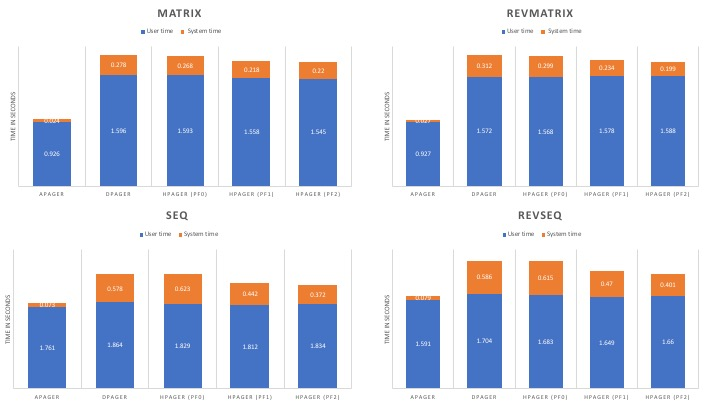
\includegraphics[scale=0.7]{Slide1.jpeg} 
	\caption{User time and system time for loaders on four benchmark programs. 
	\texttt{apager}, \texttt{dpager}, and \texttt{hpager} denote all-at-once loading, demand loading, and
hybrid loading, respectively. For hybrid loading, \texttt{pf0}, \texttt{pf1}, and \texttt{pf2} represent the number of additional page prefetching, which are 0, 1, 2 respectively. The results are averaged over 10 trails.}
	\label{bench}
\end{figure}

In both \texttt{matrix} benchmark and \texttt{revmatrix} benchmark, user time of all-at-once loading is significantly better than any other loader with different page loading strategy. Demand loading and hybrid loading have similar user time. However, prefetching pages in hybrid loading still performs better than demand loading, even the difference is relative small. This observation meets the expectation as the memory is accessed in either row or column order, and the inner loop of memory access resembles arithmetic sequence access. In terms of memory usage, demand loading performs better than both all-at-once loading and hybrid loading.

When accessing memory in an array in both forward direction and reverse direction (e.g., \texttt{seq} and \texttt{revseq}), user time of all loaders perform relatively the same but all-at-once loading performs slightly better. In terms of system time, all-at-once loading performs significantly better than the rest. This is mainly due to that many \texttt{mmap} calls are invoked with small region length in demand loading.  We find that demand loading and hybrid loading without any prefetching have relatively same performance. This is because segments except \texttt{.bss} section are usually small, which can be filled into serveral pages. Demand loading of these pages does not lead to visible overhead. In addition, prefetching more pages likely have better performance, which meets our heuristic expectation of sequential memory access. In terms of memory usage, demand loading uses less memory than all-at-once loading, again.

Based on these benchmarks, we conclude that all-at-once loading performs better than demand loading and hybrid loading in terms of runtime. However, demand loading has advantage in saving memory usage. Prefetching with more pages can have better performance in terms of runtime.

\end{spacing}
\bibliographystyle{ieeetr}
\bibliography{report}
\end{document}

